\PassOptionsToPackage{unicode=true}{hyperref} % options for packages loaded elsewhere
\PassOptionsToPackage{hyphens}{url}
%
\documentclass[10pt,ignorenonframetext,]{beamer}
\setbeamertemplate{caption}[numbered]
\setbeamertemplate{caption label separator}{: }
\setbeamercolor{caption name}{fg=normal text.fg}
\beamertemplatenavigationsymbolsempty
\usepackage{lmodern}
\usepackage{amssymb,amsmath}
\usepackage{ifxetex,ifluatex}
\usepackage{fixltx2e} % provides \textsubscript
\ifnum 0\ifxetex 1\fi\ifluatex 1\fi=0 % if pdftex
  \usepackage[T1]{fontenc}
  \usepackage[utf8]{inputenc}
  \usepackage{textcomp} % provides euro and other symbols
\else % if luatex or xelatex
  \usepackage{unicode-math}
  \defaultfontfeatures{Ligatures=TeX,Scale=MatchLowercase}
\fi
% use upquote if available, for straight quotes in verbatim environments
\IfFileExists{upquote.sty}{\usepackage{upquote}}{}
% use microtype if available
\IfFileExists{microtype.sty}{%
\usepackage[]{microtype}
\UseMicrotypeSet[protrusion]{basicmath} % disable protrusion for tt fonts
}{}
\IfFileExists{parskip.sty}{%
\usepackage{parskip}
}{% else
\setlength{\parindent}{0pt}
\setlength{\parskip}{6pt plus 2pt minus 1pt}
}
\usepackage{hyperref}
\hypersetup{
            pdftitle={Analysis of Noisy Gradient-Descent Bit Flipping (NGDBF) Decoding Algorithm},
            pdfauthor={Eric Reiss},
            pdfborder={0 0 0},
            breaklinks=true}
\urlstyle{same}  % don't use monospace font for urls
\newif\ifbibliography
\usepackage{graphicx,grffile}
\makeatletter
\def\maxwidth{\ifdim\Gin@nat@width>\linewidth\linewidth\else\Gin@nat@width\fi}
\def\maxheight{\ifdim\Gin@nat@height>\textheight\textheight\else\Gin@nat@height\fi}
\makeatother
% Scale images if necessary, so that they will not overflow the page
% margins by default, and it is still possible to overwrite the defaults
% using explicit options in \includegraphics[width, height, ...]{}
\setkeys{Gin}{width=\maxwidth,height=\maxheight,keepaspectratio}
% Prevent slide breaks in the middle of a paragraph:
\widowpenalties 1 10000
\raggedbottom
\setbeamertemplate{part page}{
\centering
\begin{beamercolorbox}[sep=16pt,center]{part title}
  \usebeamerfont{part title}\insertpart\par
\end{beamercolorbox}
}
\setbeamertemplate{section page}{
\centering
\begin{beamercolorbox}[sep=12pt,center]{part title}
  \usebeamerfont{section title}\insertsection\par
\end{beamercolorbox}
}
\setbeamertemplate{subsection page}{
\centering
\begin{beamercolorbox}[sep=8pt,center]{part title}
  \usebeamerfont{subsection title}\insertsubsection\par
\end{beamercolorbox}
}
\AtBeginPart{
  \frame{\partpage}
}
\AtBeginSection{
  \ifbibliography
  \else
    \frame{\sectionpage}
  \fi
}
\AtBeginSubsection{
  \frame{\subsectionpage}
}
\setlength{\emergencystretch}{3em}  % prevent overfull lines
\providecommand{\tightlist}{%
  \setlength{\itemsep}{0pt}\setlength{\parskip}{0pt}}
\setcounter{secnumdepth}{0}

% set default figure placement to htbp
\makeatletter
\def\fps@figure{htbp}
\makeatother


\title{Analysis of Noisy Gradient-Descent Bit Flipping (NGDBF) Decoding
Algorithm}
\providecommand{\subtitle}[1]{}
\subtitle{Using MATLAB/Octave and the PRISM Model Checking Tool}
\author{Eric Reiss}
\date{}


\usepackage[most]{tcolorbox}

\tcbset{
  frame code={},
  center title,
  left=0pt,
  right=0pt,
  top=0pt,
  bottom=0pt,
  colback=blue!20,
  colframe=white,
  width=\dimexpr\textwidth\relax,
  enlarge left by=0mm,
  boxsep=5pt,
  arc=0pt,outer arc=0pt,
}


\pgfdeclareimage[]{mybackground}{figures/OldMainTower.png}

\setbeamertemplate{title page}{

  \begin{picture}(0,0)
    
     \put(50,-100){%
      \pgfuseimage{mybackground}
    }
     
    \put(0,-40.7){%
      \begin{minipage}[b][45mm][t]{226mm}
        \usebeamerfont{title}{\inserttitle\par}
        \usebeamerfont{subtitle}{\insertsubtitle\par}
        \vspace{0.5cm}
        \usebeamerfont{author}{\insertauthor\par}
        \usebeamerfont{author}{Utah State University\par}
      \end{minipage}
    }
    
  \end{picture}
}


\setbeamertemplate{itemize/enumerate subbody begin}{\vspace{0.125cm}\begin{tcolorbox}[colback=red!20]}
\setbeamertemplate{itemize/enumerate subbody end}{\end{tcolorbox}\vspace{0.125cm}}
\setbeamertemplate{itemize/enumerate body begin}{\vspace{0.125cm}\begin{tcolorbox}}
\setbeamertemplate{itemize/enumerate body end}{\end{tcolorbox}\vspace{0.125cm}}
\setbeamertemplate{itemize/enumerate item end}{\vspace{0.125cm}}

\setlength{\itemsep}{0.5cm}

\makeatletter
\addtobeamertemplate{itemize begin}{
\def\@listi{\leftmargin\leftmargini
              \topsep    0pt
              \parsep    0pt
              \itemsep   3pt plus 2pt minus 3pt}
\partopsep 0pt
}
\makeatother



\begin{document}
\frame{\titlepage}

\begin{frame}{Overview}
\protect\hypertarget{overview}{}
\begin{itemize}[<+->]
\tightlist
\item
  LDPC Codes and Trapping Sets
\item
  Algorithm Overview
\item
  Model Construction
\item
  MATLAB/Octave Tool Overview
\item
  Sample Generation
\item
  Energy Calculation
\item
  Transisition Probabilities
\item
  Write Files and Process Output
\item
  What's Next
\item
  Sources
\end{itemize}
\end{frame}

\begin{frame}{LDPC Codes and Trapping Sets}
\protect\hypertarget{ldpc-codes-and-trapping-sets}{}
\begin{itemize}[<+->]
\tightlist
\item
  Low-Density Parity Check (LDPC) codes were introduced by Gallager in
  1963
\item
  LDPC codes are commonly represented as sparse Tanner graph
\item
  Trapping sets are a sub-set of the graph that limit the performance of
  decoding algorithms, creating an error-floor
\item
  Absorbing sets are a special case of a trapping sets that are stable
  in a bit flipping decoder {[}1{]}
\end{itemize}

\begin{figure}
\centering
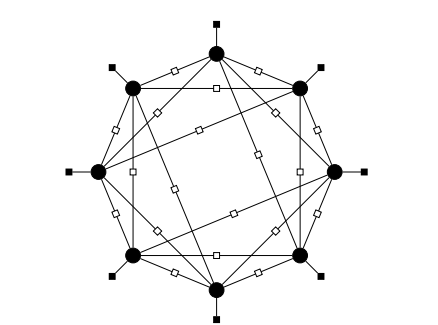
\includegraphics[width=0.2\textwidth,height=\textheight]{figures/8_8_absorbing.png}
\caption{(8,8) Absorbing set that is dominant in the 802.3an 10GBASE-T
LDPC Code {[}2{]}.}
\end{figure}
\end{frame}

\begin{frame}{Algorithm Overview}
\protect\hypertarget{algorithm-overview}{}
\begin{itemize}[<+->]
\tightlist
\item
  NGDBF is part of a family of bit flipping decoding algorithms
\item
  Improves upon the Gradient-Descent Bit Flipping (GDBF) Decoding
  Algorithm proposed by Wadayama et al.~{[}3{]}

  \begin{itemize}[<+->]
  \tightlist
  \item
    GDBF gets ``stuck'' in local minima while decoding
  \end{itemize}
\item
  NGDBF introduces psuedo-random noise to escape local minima
\item
  Algorithm steps {[}4{]}:

  \begin{itemize}[<+->]
  \tightlist
  \item
    Let \(H\) be an \(n\times m\) parity check matrix, \(N_i\) be the
    adjacency for bit \(i\), \(M_j\) be the adjacency for parity check
    \(j\)
  \item
    Given channel samples, \(\vec{y}\), initialize \(\vec{x}\) to be the
    \(sign(\vec{y})\)
  \item
    Compute the syndrome, \(s_j = \prod_{i\in M_j}x_i\)
  \item
    Calculate the energy for bit i,
    \(E_i = y_ix_i+w\sum_{j\in N_i}s_j + z_i\), where w is i.i.d white
    noise and \(z_i\) is a zero mean noise pertubation
  \item
    Given a threshold \(\theta\) flip bit \(i\) if \(E_i < \theta\)
  \end{itemize}
\end{itemize}

\begin{figure}
\centering
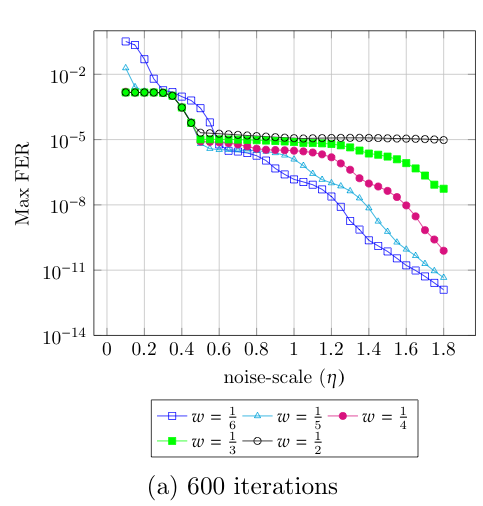
\includegraphics{figures/thumbnail_Ngdbf-error-floor.cgi.png}
\caption{FER Graph from {[}1{]} at 600 iterations}
\end{figure}
\end{frame}

\begin{frame}{Model Construction}
\protect\hypertarget{model-construction}{}
\begin{itemize}[<+->]
\tightlist
\item
  The Markov Chain structure used in the tool was proposed in {[}1{]}
\item
  For a given (a,b) trapping set, the state space is described by the
  a-bit binary representation of the numbers from 0 to \(2^a-1\)

  \begin{itemize}[<+->]
  \tightlist
  \item
    For example, the (3,3) trapping set would have 8 states, 000 - 111
  \item
    A transition from 010 to 000 implies that the middle bit flipped
  \end{itemize}
\item
  Edge probabilities are calculated by first calculating the probability
  that a bit flips using the cdf centered on the energy function with
  the noise pertubation subtracted

  \begin{itemize}[<+->]
  \tightlist
  \item
    \(P_{flip} = normcdf(\theta,E_i,\sigma)\)
  \end{itemize}
\item
  The prbability of a transistion is then calculated by multiplying the
  flip probabilities

  \begin{itemize}[<+->]
  \tightlist
  \item
    For example, state 010 to 100, where a state is \(b_2b_1b_0\), is
    calculated by
    \(P_{010\rightarrow 100}=P_{b_2flip}*P_{b_1flip}*(1-P_{b_0flip})\)
  \end{itemize}
\end{itemize}
\end{frame}

\begin{frame}{MATLAB/Octave Tool Overiview}
\protect\hypertarget{matlaboctave-tool-overiview}{}
\begin{itemize}[<+->]
\tightlist
\item
  This tool will hopefully automate all the manual calculations that
  were performed in T. Tithi's dissertation {[}1{]}
\item
  Located in the USU\_stochastic\_case\_studies repository in the
  ngdbf\_models folders, contains the following files

  \begin{itemize}[<+->]
  \tightlist
  \item
    run\_ngdbf.m: Driver function that contains most of the relevant
    code
  \item
    load\_trapping\_sets.m: Script containing some of the trapping sets
    in University of Arizona's Trapping Set Ontology {[}5{]}.
  \item
    write\_model.m: Helper function that takes data from run\_ngdbf to
    write a PRISM model
  \item
    write\_explicit\_model.m: Helper function that creates the necessary
    files to generate an explicit PRISM model
  \item
    isOctave.m: Helper function to determine if the script is running on
    Octave or MATLAB
  \item
    get\_error\_sample\_size.m: Helper function to calculate the number
    of error samples needed
  \end{itemize}
\item
  The tool uses channel information to programmatically generate a model
  of the algorithm for each possible initial state
\item
  Four main sections of the run\_ngdbf.m are

  \begin{itemize}[<+->]
  \tightlist
  \item
    Generate samples
  \item
    Calculate all energy values
  \item
    Calculate transition probabilities
  \item
    Write files and process PRISM output
  \end{itemize}
\end{itemize}
\end{frame}

\begin{frame}[fragile]{Sample Generation}
\protect\hypertarget{sample-generation}{}
\begin{itemize}[<+->]
\tightlist
\item
  Samples are pulled from Gaussian distribution with a mean of \(1\) and
  a standard deviation of \(\sigma=\sqrt{\frac{1}{R*10^{SNR/10}}}\),
  where \(R\) is the code rate
\item
  Currently the tool generates a list of samples and sorts into valid
  and error sample bins
\item
  An error sample is one that comes from the negative tail of the
  Gaussian distribution
\item
  There is probably a better way to do this, and finding that is on the
  to-do list
\end{itemize}

\begin{verbatim}
loop_check = get_error_sample_size(sym_size);
valid_samples = zeros(1,loop_check); % initialize valid samples
valid_idx = 1;
error_samples = zeros(1,loop_check); % initialize error samples
error_idx = 1;
while valid_idx <= loop_check || error_idx <= loop_check 
   temp = normrnd(1,sigma); % generate samples
   if temp > 0 % sort valid samples
      valid_samples(valid_idx) = temp;
      valid_idx = valid_idx +1;
   end
   if temp < 0 % sort error samples
      error_samples(error_idx) = temp;
      error_idx = error_idx+1;
   end
end
\end{verbatim}
\end{frame}

\begin{frame}[fragile]{Energy Calculation}
\protect\hypertarget{energy-calculation}{}
\begin{itemize}[<+->]
\tightlist
\item
  To create the model, all possible energy values must be calculated
\item
  The syndrome, called chk\_nodes here, is also calculated
\end{itemize}

\begin{verbatim}
%initialize Energy and check node matrices
E = zeros(2^sym_size,sym_size);
chk_nodes = ones(1, check_size);
chk_sum = zeros(1,sym_size);
% Calculate all possible energy values for each state
for row = 1:2^sym_size
   % Calculate all check nodes
   for adj_row = 1:check_size
         for adj_col = 1:sym_size
            if adj_mat(adj_row,adj_col) == 1
               chk_nodes(adj_row) = chk_nodes(adj_row)*x(row,adj_col);
               chk_sum(adj_col) = chk_sum(adj_col)+chk_nodes(adj_row);
            end
         end
   end
   % Calculate energy values
   for E_idx = 1:sym_size
         E(row,E_idx) = y(E_idx)*x(row,E_idx)+w*chk_sum(E_idx);
   end
end
\end{verbatim}
\end{frame}

\begin{frame}[fragile]{Transition Probabilities}
\protect\hypertarget{transition-probabilities}{}
\begin{itemize}[<+->]
\tightlist
\item
  Using the energy calculations, the transistion matrix is generated
\end{itemize}

\begin{verbatim}
p = ones(2^sym_size,2^sym_size);
% Flip probabilities calculated according to Eq 3.13 in T. Tithi
% dissertation (pg. 26)
for row = 1:2^sym_size
   px = zeros(1,sym_size);
   for p_idx = 1:sym_size
         px(p_idx) = normcdf(theta,E(row,p_idx),sigma);
   end
   rowbin = dec2bin(row-1,sym_size);
   for col = 1:2^sym_size
         colbin = dec2bin(col-1,sym_size);
         for p_idx = 1:sym_size
            if rowbin(p_idx) == colbin(p_idx)
               p(row,col) = p(row,col)*(1-px(p_idx));
            else
               p(row,col) = p(row,col)*px(p_idx);
            end
         end
   end
end
% Sanity check
if sum(round(sum(p.'))) ~= 2^sym_size
   fprintf("Error: Probabilities do not sum to 1\n");
   return;
end
\end{verbatim}
\end{frame}

\begin{frame}[fragile]{Write Files and Process Outputs}
\protect\hypertarget{write-files-and-process-outputs}{}
\begin{itemize}[<+->]
\tightlist
\item
  The model is written using the helper functions write\_model.m and
  write\_explicit\_model.m
\item
  A system call to PRISM runs either a transient analysis, steady-state
  analysis, or a user-defined property analysis
\item
  The result is saved for transient and steady-state analysis

  \begin{itemize}[<+->]
  \tightlist
  \item
    It works with some properties, but this needs to be expanded
  \end{itemize}
\end{itemize}

\begin{verbatim}
% Process Output for transient and steady state
if (tag(3) == 't' && tag(4) == 'r') || (tag(3) == 's' && tag(4) == 's')
      str_idx = regexp(output,regexptranslate('wildcard','0:\(*\)=*'));
      output = substr(output,str_idx);
      split_output = strsplit(output,"\n"); 
      for out_idx = 1:2^sym_size
         str_to_parse = char(split_output(out_idx));
         if (str_to_parse(1) >= "0") && (str_to_parse(1) <= "9")
            temp = textscan(str_to_parse,"%d:(%d)=%f");
            state_temp = temp{1,2};
            p_out(idx,state_temp+1) = temp{1,3};
         else
            break; 
         end
      end
elseif tag(3) == 'p'
      str_idx = strfind(output,"Result");
      output = substr(output,str_idx);
      p_temp = textscan(output,"Result: %f (exact floating point)");
      p_out(idx,1) = p_temp{1,1};
else
      % Do nothing
end
fprintf(file_out,"initial state: %d\n%s\n----------------------------------------------------------------------------------------------------\n\n",istate,output);
\end{verbatim}
\end{frame}

\begin{frame}{What's Next}
\protect\hypertarget{whats-next}{}
\begin{itemize}[<+->]
\tightlist
\item
  Issues and Possible Solutions

  \begin{itemize}[<+->]
  \tightlist
  \item
    Runtime

    \begin{itemize}[<+->]
    \tightlist
    \item
      Large trapping sets take a long time to run
    \item
      Maybe rewrite in C?
    \item
      Need to determine if PRISM is slow or just file I/O
    \end{itemize}
  \item
    Sample generation

    \begin{itemize}[<+->]
    \tightlist
    \item
      Also takes a long time for large trapping sets
    \item
      Maybe use some kind IS?
    \end{itemize}
  \end{itemize}
\item
  To do

  \begin{itemize}[<+->]
  \tightlist
  \item
    Use PRISM output to generate FER graphs

    \begin{itemize}[<+->]
    \tightlist
    \item
      May need to run more simulations for each initial state and take
      average?
    \end{itemize}
  \item
    Validate tool against Tasnuva's dissertation results
  \end{itemize}
\end{itemize}
\end{frame}

\begin{frame}{Sources}
\protect\hypertarget{sources}{}
\begin{itemize}[<+->]
\tightlist
\item
  {[}1{]} T. Tithi, ``Error-Floors of the 802.3an LDPC Code for Noise
  Assisted Decoding'', \emph{All Graduate Theses and Dissertations},
  pp.~7465, 2019.
\item
  {[}2{]} T. Tithi, C. Winstead, and G. Sundararajan, ``Decoding LDPC
  codes via Noisy Gradient Descent Bit-Flipping with Re-Decoding'',
  2015.
\item
  {[}3{]} T. Wadayama, K. Nakamura, M. Yagita, Y. Funahashi, S. Usami,
  and I. Takumi, ``Gradient descent bit flipping algorithms for decoding
  LDPC codes'', \emph{Communications, IEEE Transactions on}, vol.~58,
  no. 6, pp.~1610-1614, 2010.
\item
  {[}4{]} C. Winstead and E. Boutillon, ``Hardware Demonstration of
  Noisy Gradient Descent Bit Flipping (NGDBF) for IEEE 802.3 Standard
  Code''.
\item
  {[}5{]} ``Trapping Set Ontology'',
  https://uweb.engr.arizona.edu/\textasciitilde vasiclab/Projects/CodingTheory/TrappingSetOntology.html
  (accessed Aug 4, 2023).
\end{itemize}
\end{frame}

\end{document}
